\chapter{Experimental Analysis}
\label{sec:exp}

The following is a description of the environment that has been set up for the fault injection tests, using chosen benchmark applications and the hardware design preparation behind the related choices. The second part of this chapter illustrates in detail the obtained experimental results, highlighting some interesting considerations.

\section{Fault Injection Environment}

Before proceeding with the fault injection campaign, which aims to demonstrate the effectiveness of the developed fault tolerance design, the Fault Injection Tool requires some extra hardware for a good understanding of the obtained results.

\subsubsection{Watchdog Configuration}
The watchdog IP, during the design stage, is configured through its customization wizard with a default timeout value of 2 seconds (two times the clock frequency) and it is started by default. This choice has been taken because under normal operational conditions, the MicroBlaze is capable of starting the watchdog and setting a correct timeout value.\bigskip
 
Instead, with the chosen fault injection method, the MicroBlaze directly starts with a bit-flip in his configuration, hence it may be not able to start correctly the watchdog or set a valid timeout value. Therefore, the campaign results would not be valid.\bigskip

\subsubsection{Hardware to count the number of timeouts}
In order to understand if the watchdog is capable of covering a good number of faults by expiring, the design has been equipped with a UP counter. The counter is reset once at each FGPA programming with a new full bitstream. The counter is incremented every time the watchdog expires by connecting the CLK port to the timeout signal, and its value is obtained via an AXI GPIO peripheral that is connected to the AXI Interconnect. \bigskip

\begin{figure}[H]
\centering
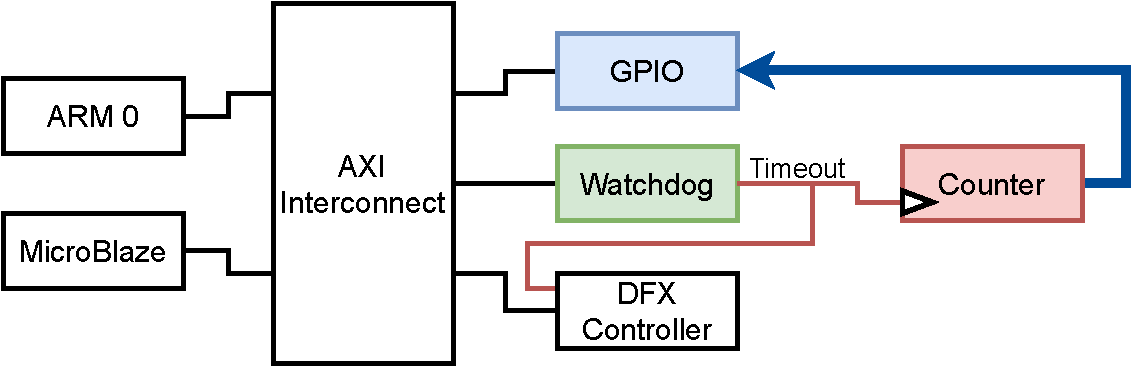
\includegraphics[width=0.95\linewidth]{images/chapter5/upc.pdf}
\caption{Hardware schematic to count the number of times the watchdog time outs.}
\end{figure}

Both the MicroBlaze and the PS can access it. Because the MicroBlaze is under test and may not be able to access correctly the GPIO peripheral, the value is read from one of the ARM cores in the PS side.\bigskip

% UP-counter added to read the number of times the reconf is triggered (clk connected to trigger). Count accessed via a GPIO memory mapped from the ARM core.

\subsubsection{Benchmark Firmware}

As explained in previous sections, a good benchmark software is required for a good fault injection campaign for two reasons:
\begin{itemize}
    \item A good benchmark software can stress various aspects of the MicroBlaze's hardware (ALU, Decode Unit, Controller Unit, etc.) and reveal a hidden fault.
    \item A good benchmark software can self-test itself (checking the correctness of the produced results) and trigger the reconfiguration when needed.
\end{itemize}

The following is an extract of the firmware running on the MicroBlaze, that computes the Fibonacci series up to a certain point and checks the results via a simple checksum check:

\begin{lstlisting}[style=C]
int main() {
  int i;
  uint64_t op1 = 0, op2 = 0, res = 0, checksum = 0;
  GBcnCtrl hBcn;

  i = XPAR_BEACON_WATCHDOG_0_S00_AXI_BASEADDR;
  GBcnCtrl_Initialize(&hBcn, i);

  print("started? ", GBcnCtrl_IsStarted(&hBcn) ? 1 : -1);
  i = hBcn.modules->module0.DATAREG;
  print("timeout: ", i ? i : -1);
  GBcnCtrl_SetTimeoutValue(&hBcn, XPAR_CPU_CORE_CLOCK_FREQ_HZ<<1);
  GBcnCtrl_Start(&hBcn);
  print("started? ", GBcnCtrl_IsStarted(&hBcn) ? 1 : -1);
  i = hBcn.modules->module0.DATAREG;
  print("timeout: ", i ? i : -1);

  op1 = op2 = 1;
  print("Fibonacci current value ", op1);
  print("Fibonacci current value ", op2);

  while(1) {
    checksum ^= (res = op1 + op2);
    if(res > 0xfffff) {
  	  res = 1;
  	  op2 = 0;
  	  print("\n\rDONE_1 DONE_1 DONE_1\r\n");
  	  break;
    }

    print("Fibonacci current value ", (uint64_t)res);
    op1 = op2;
    op2 = res;
    for (i = 0; i < 1e5; i++); // a bit of delay
    GBcnCtrl_Toggle(&hBcn);
  }

  printt("CHECKSUM: ", checksum);
  if (checksum == 1673873) {
    print("DONE_2 DONE_2 DONE_2\r\n");
    for (i = 0; i < 5e6; i++); // delay
    GBcnCtrl_Toggle(&hBcn); // all fine!
  } else {
    print("WRONG CHECKSUM!\r\n");
    while(1); // stops toggling because wrong checksum
  }
}
\end{lstlisting}

\subsubsection{How the fault injection tool access the number of expired times}

The Fault Injection Tool has been enhanced to support the retrieval of the number of times the watchdog expires at each run. It does it via an XSCT script that appends in a file the retrieved number, as follows:\bigskip

\begin{lstlisting}[style=tcl]
connect -url tcp:127.0.0.1:3121

# selects the ARM #0 core
targets -set -nocase -filter {name =~ "*A9*#0"} 
set outfile1 [open "faulty_bitstreams/uB_results/dfx_cnt.txt" a+]    

# reads the value from the GPIO register
puts $outfile1 [mrd -value 0x41200008 1] 
close $outfile1
\end{lstlisting}

\subsection{Watchdog Inhibition}
In some cases may be useful to inhibit the watchdog. This allows to detach the timeout signal from the DFX Controller, thus the reconfiguration is not triggered. This is useful for example to debug the firmware. In this case, the firmware stops kicking the watchdog during the interruption of the software and thus the MicroBlaze is automatically reconfigured and restarted. To allows the inhibition by toggling a physical switch on the board, the following is the used hardware scheme:

\begin{figure}[H]
\centering
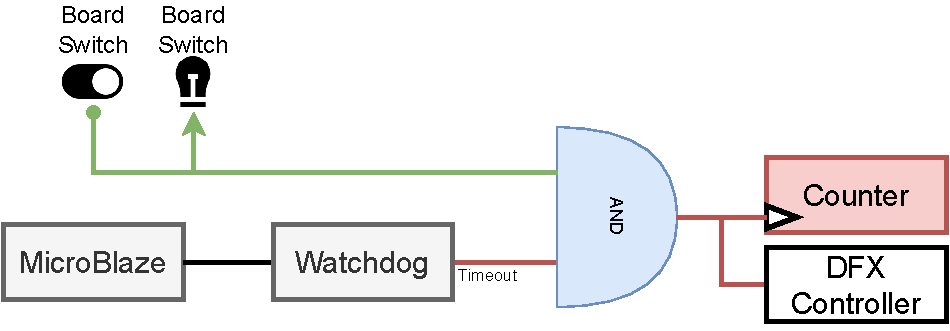
\includegraphics[width=0.95\linewidth]{images/chapter5/btn.pdf}
\caption{Hardware schematic to inhibit the watchdog using a physical switch.}
\end{figure}


% FI tool generates bitstream -> for each run
% pre\_tcl script to program the bitsteam and the ELF
% post\_tcl to launch the microblaze execution (con comand)
% cnt\_tcl script to obtain the number of reconfigurations triggered (reads from the GPIO mrd 0x41200008)

\section{Experimental Results}

In this section, the main obtained results are presented and discussed. During the overall test period, ten campaigns of fault injection have been performed. Each campaign is made of 100 injections. Some of them are aborted, thus the mean number of completed injections per run is around 96, leading to a total of 966 injections. \bigskip

For each fault, there can be three possible outcomes, and each one can have a different reason behind it:
\begin{itemize}
    \item Correct result:
    \begin{enumerate}
        \item The fault has not been excited by the software so it is naturally masked and the result is automatically correct.
        \item The fault caused a CPU halt (no detected output on the UART). The system corrected the fault and the final output is correct. It is identical to the golden one, hence it is marked as correct.
    \end{enumerate}
    \item The output is different from the golden one (SDE):
    \begin{enumerate}
        \item The fault has not been detected by the watchdog, thus it is not fixed.
        \item The MicroBlaze noticed the fault while executing the program and printing messages and it has been fixed. However, the output is different from the golden one, even if the final result is correct. Marked as SDE anyway. An example is shown in Appendix \ref{sec:sde_output}.
        \item The MicroBlaze noticed the fault and tried to fix it, unsuccessfully. The output is different and the result remained incorrect.
    \end{enumerate}
    \item The MicroBlaze is halted:
    \begin{enumerate}
        \item The hang is detected by the watchdog, but it could not be fixed.
        \item The MicroBlaze does not output anything on the UART, even if the watchdog is kicked correctly. No output means that the CPU is in the hang state but a correct kicking act means that the CPU is working so the reconfiguration is not triggered.
    \end{enumerate}
\end{itemize}

\newpage
The following one is a summary of the obtained results from the conducted campaigns:

\begin{figure}[H]
\centering
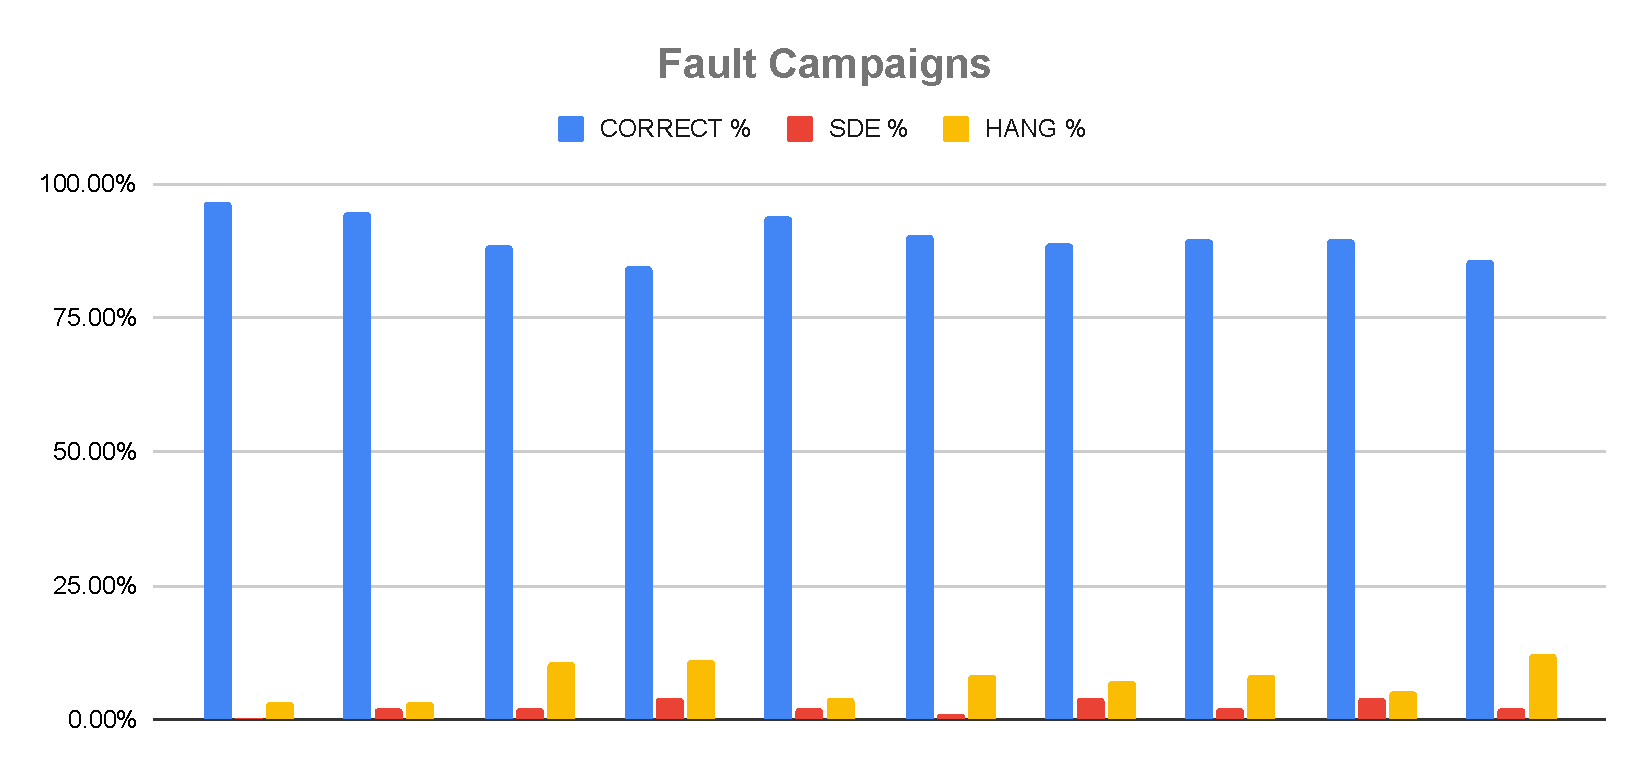
\includegraphics[width=0.95\linewidth]{images/chapter5/mchart.pdf}
\caption{Chart representing the executed Fault Injection campaigns.}
\end{figure}

Each value is represented as the percentage of the total number of injections for each campaign. The blue ones represent the correct results. The overall correct results among all the campaigns are 872, 27 of which have been corrected by the fault tolerance system. \bigskip

Among the red ones representing SDEs, the total is 23. Among these 23 SDEs, 11 have been successfully corrected, while the other 12 have not been corrected. Among those 12 not corrected SDEs, 1 has been detected but the system could not fix them, while the remaining 11 have not been detected at all. This can be easily fixed by increasing the quality of self-test routines in the firmware, looking for example for differences in the produced UART output and the expected one or by comparing written memory values with the expected ones. Consequently, this may help in increasing the coverage of those faults. \bigskip

The remaining yellow cases represent situations where the MicroBlaze is completely halted, even 1fter one or multiple reconfigurations have been performed. There is a total of 71 hangs, 1 of which has not been detected at all. As the not detected SDEs, this can be fixed by increasing the quality of self-test routines. The remaining cases are the uncoverable ones. \bigskip

Those values are presented in the following charts:

\begin{figure}[H]
  \centering
  \begin{minipage}[t]{.49\linewidth}
  \begin{figure}[H]
  \centering
    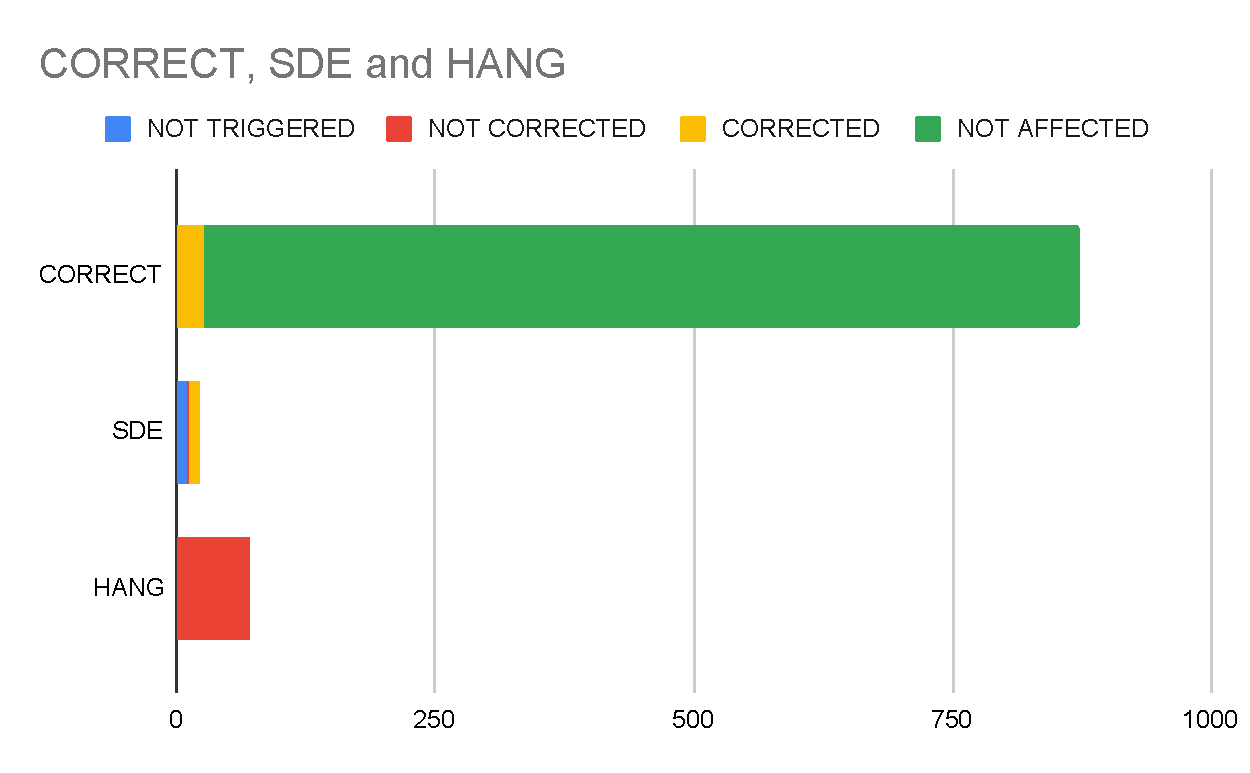
\includegraphics[width=\linewidth]{images/chapter5/csh1.pdf}
    % \caption{HI}
    % \label{fig:c}
  \end{figure}
  \end{minipage}
  \hfill
  \begin{minipage}[t]{.49\linewidth}
  \begin{figure}[H]
	\centering
	% svg inclusion, requires inkscape
    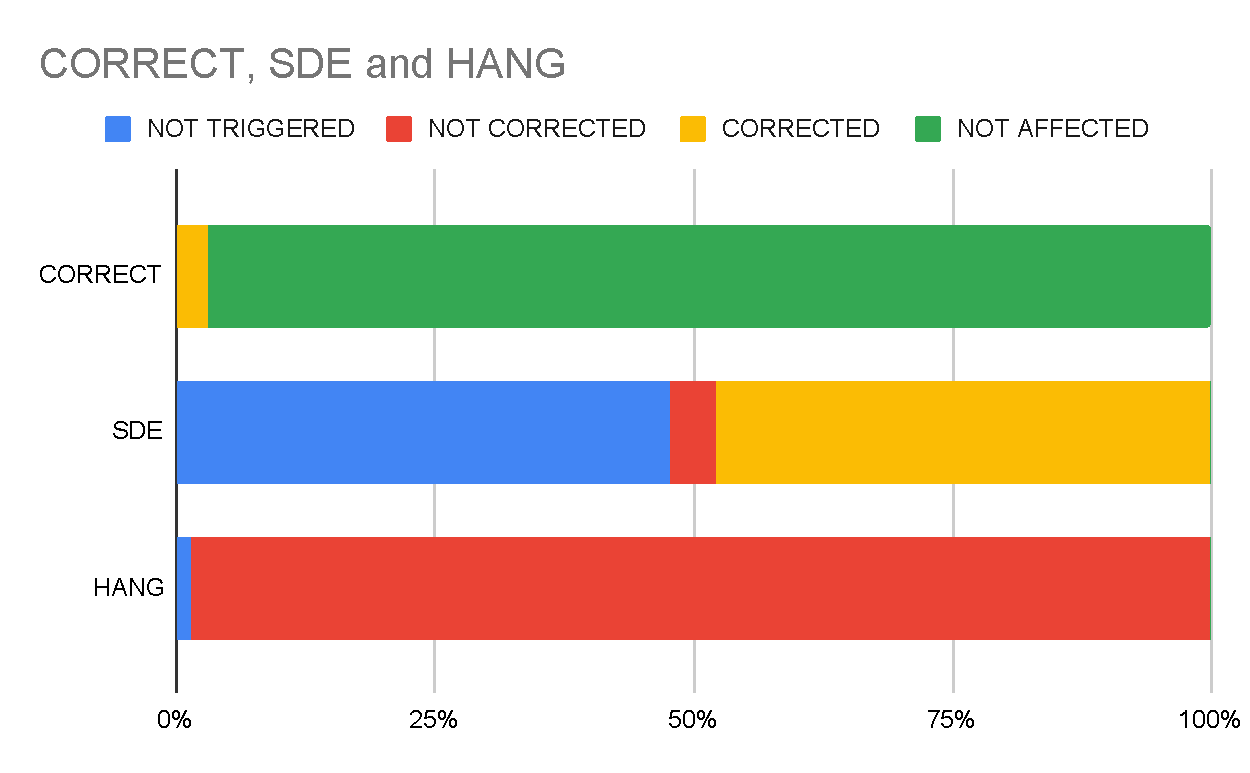
\includegraphics[width=\linewidth]{images/chapter5/csh2.pdf}
    % \caption{SVG}
    % \label{fig:svg}
  \end{figure}
  \end{minipage}
  \caption{Charts showing the times the reconfiguration is triggered (or not) and how many times it solved the issue (or not).}
\end{figure}

As a side note, the unrecoverable cases are particular cases where it is not possible to say if the overall fault tolerance system is working or not. Unfortunately, the bitstreams cannot be fully controllable and the used fault injection tool randomly injects bit flips in an area that is thought to be 100\% dedicated to the MicroBlaze. Unfortunately, in the reality it is not true: a bitflip could affect a configuration instruction instead of a configuration bit, leading to a misconfiguration anywhere else in the overall FPGA, thus it cannot be fixed by the partial reconfiguration.\bigskip

By improving the quality of the self-test routines, the fault tolerance system may be able to detect the faults and fix them. As an example, the software has been enhanced to detect errors in memory access and division or modulus operations. Those two mathematical operators are used to convert an integer into its string representation. The two operators are mutually tested at each operation by first applying the division operator then it is again multiplied by the dividend and finally the computed modulus is applied. This is the definition of the remainder. The following is the implementation:

\begin{lstlisting}[style=C]
while (a != 0) {
  /* module operation test */
  pmod = a % 10;
  if ((a / 10) * 10 + pmod != a || a - (a/10)*10 != pmod) 
    while(1); // HALT. Triggers the watchdog.
  
  str[i--] = pmod + '0';
  if (str[i + 1] - '0' != pmod) // Checks stored value
    while(1); // HALT. Triggers the watchdog.
  
  a /= 10;
}
\end{lstlisting}

In addition, the firmware checks that each character sent over the UART is the same as the one expected. This is done by comparing the expected character with the one received. If they are different, the MicroBlaze is halted, triggering the watchdog. To achieve this, the UART has been instantiated with a loopback connection from the \textit{TX} channel to the \textit{RX} channel, as follows:

\begin{figure}[H]
\centering
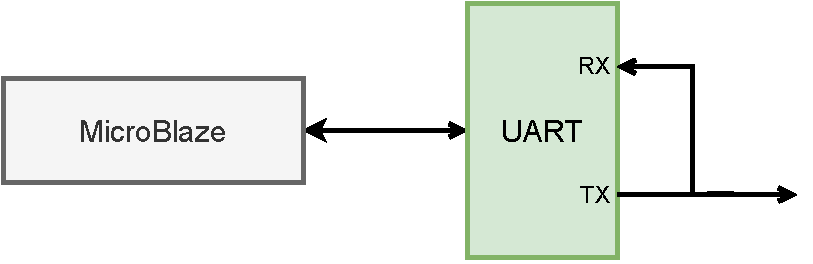
\includegraphics[width=0.95\linewidth]{images/chapter5/sch.pdf}
\caption{UART loopback schematic.}
\end{figure}

The firmware implements a custom \textit{print} routine that checks the received character and if it is different from the expected one, it triggers the watchdog. Moreover, it accesses the string memory (to send it) both with byte-oriented access and word-oriented access. The latter is used to check that the string is correctly stored in the memory and that the MicroBlaze does not have any fault in the memory access unit.

\begin{lstlisting}[style=C]
void print(char *buf) {
  int i; char *pbuf = buf; char ch, tst;

  for (i = 0; buf[i]; i++); // length computation
  while(*pbuf) {
    XUartLite_Send(phRef, (u8 *)pbuf, 1); // Send the character
    while(!XUartLite_Recv(phRef, (u8 *)&ch, sizeof ch)); // Receive the character

    /* Tests single byte memory access vs 32 bit memory access */
    pt = (u32 *)((u32)pbuf & 0xfffffffc); /* 32b aligned addr */
    tst = ((*pt >> (((pbuf - (char *)pt)) << 3)) & 0xff); 
    if (ch != *pbuf || ch != tst) while(1); // HALT.
    pbuf++; i++;
  }

  if (i || *pbuf) while(1); // just to be sure
}
\end{lstlisting}

Everything is now set and ready to be tested again. The previous 10 campaigns are executed again, with the same seeds to generate the faults. This means that the tool is able to generate again the same faults as before, thus the new firmware results can be compared with the previous ones:

\begin{figure}[H]
\centering
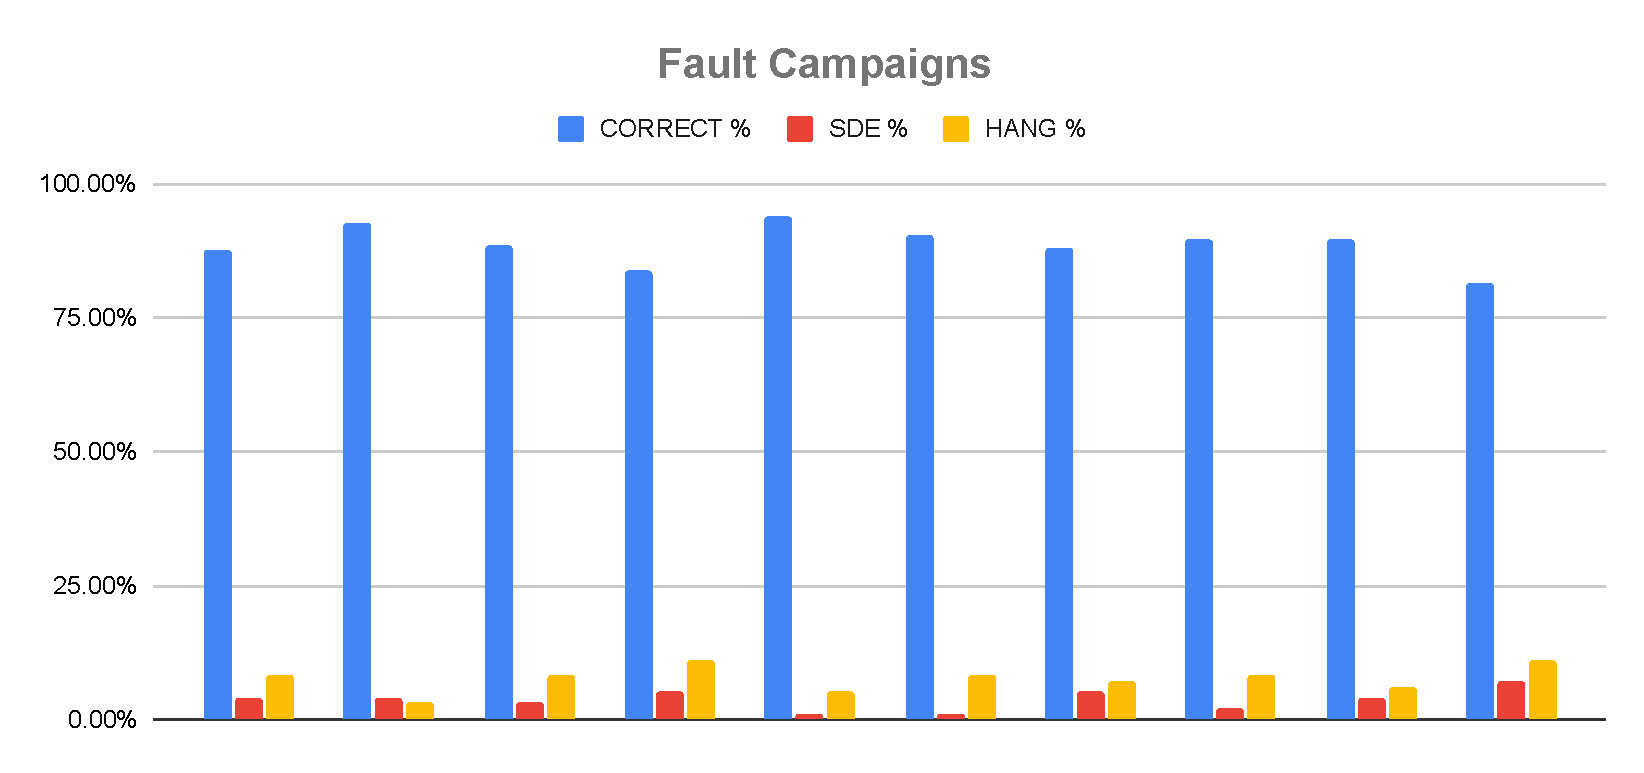
\includegraphics[width=0.95\linewidth]{images/chapter5/cici_cici.pdf}
\caption{Chart representing the repeated Fault Injection campaigns with the new firmware.}
\end{figure}

The new firmware is able to detect almost all the faults, lowering in the number of not detected among the SDEs to 1 (2.9\% among the SDEs) and to 0 among the HANGs, as shown in the following chart:

\begin{figure}[H]
  \centering
  \begin{minipage}[t]{.49\linewidth}
  \begin{figure}[H]
  \centering
    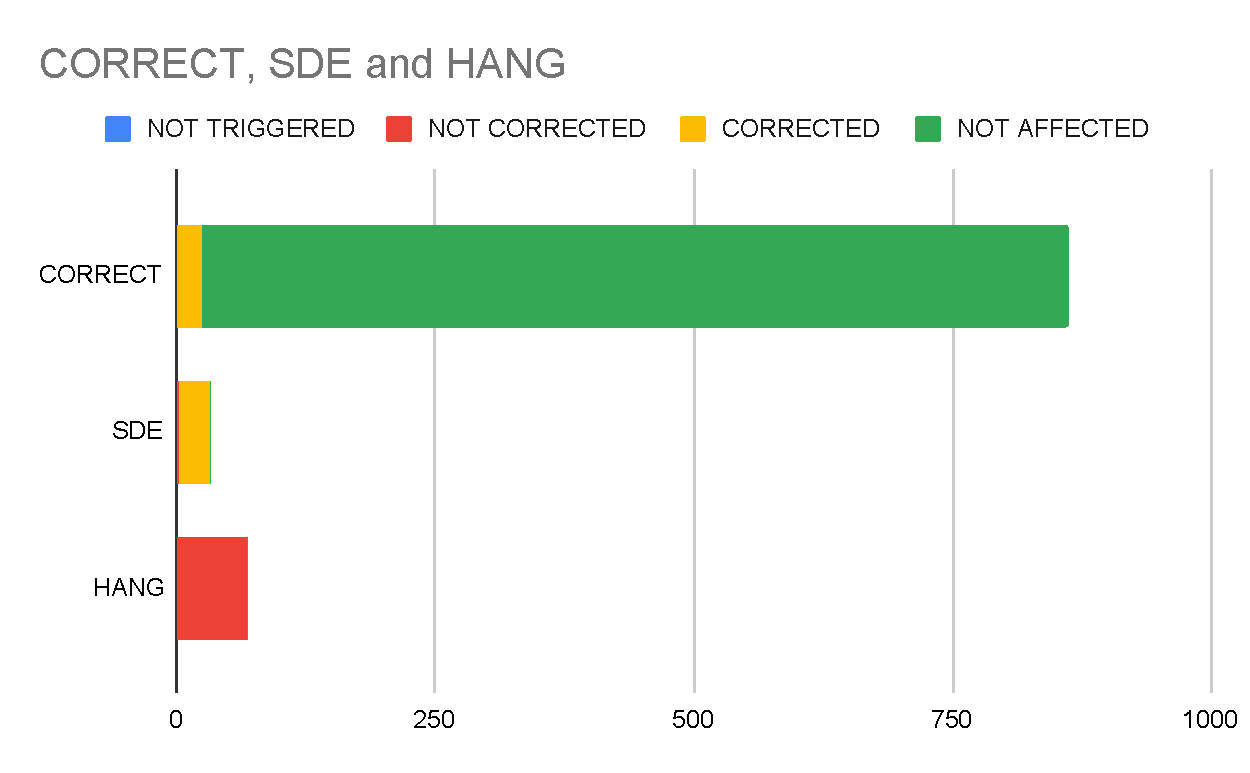
\includegraphics[width=\linewidth]{images/chapter5/csh3.pdf}
    % \caption{HI}
    % \label{fig:c}
  \end{figure}
  \end{minipage}
  \hfill
  \begin{minipage}[t]{.49\linewidth}
  \begin{figure}[H]
	\centering
	% svg inclusion, requires inkscape
    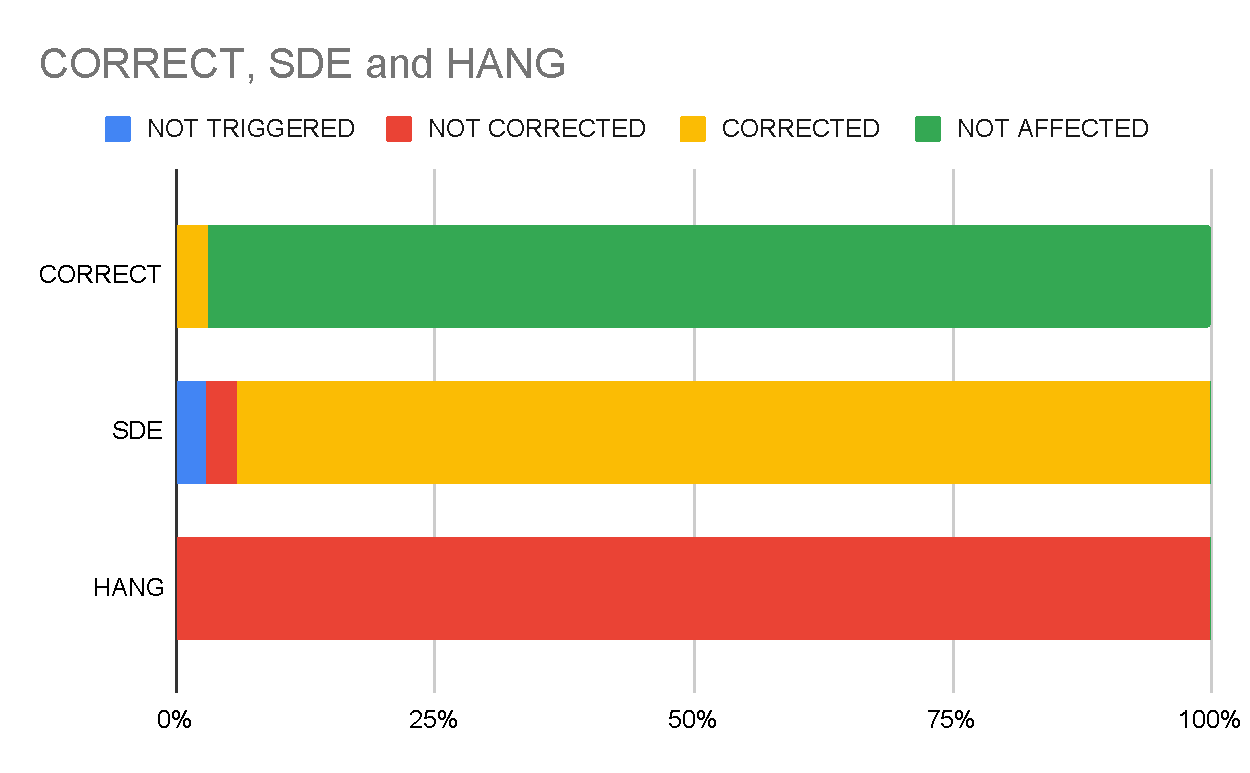
\includegraphics[width=\linewidth]{images/chapter5/csh4.pdf}
    % \caption{SVG}
    % \label{fig:svg}
  \end{figure}
  \end{minipage}
  \caption{Charts showing the times the reconfiguration is triggered (or not) and how many times it solved the issue (or not). Second run with the new firmware.}
\end{figure}
